\documentclass[a4paper, 12pt]{article}

\usepackage{graphicx} % Required for the inclusion of images
\usepackage{amsmath} % Required for some math elements 
\usepackage{times} % Uncomment to use the Times New Roman font
\usepackage{pgffor}
\title{Institute of Engineering,\\ Thapathali Campus \\ Computer Aided Drawing \\ ME 505} % Title
\author{Bibek Magar}
\date{\today} % Date for the report

\begin{document}
\maketitle % Insert the title, author and date
	\begin{center}
		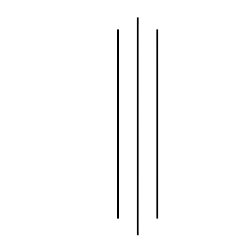
\includegraphics{gfx/lines.png}
	\end{center}
	\begin{center}
		\textbf{Tutorial for Computer Aided Drawing Lab}
	\end{center}
	
	\newpage
%lab 1
\section{lab 1: Introduction to AutoCAD interface and coordinate systems}
\begin{center}
	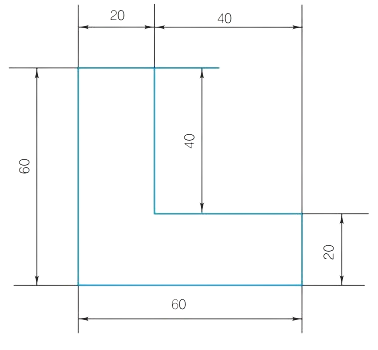
\includegraphics{gfx/fig.png}
\end{center}
\emph{Assume absolute coordinate of the bottom left corner be (15, 15).}
\subsection{Draw the given figure in AutoCAD using the absolute coordinates and write the command sequence.}
\subsection{Draw the given figure in AutoCAD using the relative coordinates and write the command sequence.}
\subsection{Draw the given figure in AutoCAD using the relative polar coordinates and write the command sequence.}
\clearpage
%lab2
\section{lab 2: Introduction to AutoCAD sketch tools}
\subsection{Draw a parabola with double ordinate 100 mm and axis 60 mm. }
\foreach \i in {2,...,3}{
	\subsection{Draw the given figure in AutoCAD and write the command sequence.}
	\begin{center}
    	\includegraphics[width = 17cm]{gfx/l2t\i.PNG}
	\end{center}
}
\clearpage
%lab 3
\section{Lab 3: Introduction to AutoCAD modify tools}
\foreach \n in {1,...,6}{
	\subsection{Draw the given figure in AutoCAD and write the command sequence.}
	\begin{center}
		\includegraphics[scale= 0.6]{gfx/l3t\n.png}
	\end{center}
}
\clearpage
%lab 4
\section{Lab 4: 2D Drafting I}
\foreach \n in {1,...,3}{
	\subsection{Draw the given figure in AutoCAD and write the command sequence.}
	\begin{center}
		\includegraphics[width = 12cm, height = 10cm]{gfx/l4t\n.PNG}
	\end{center}
}
%lab 5
\section{Lab 5: 2D Drafting II: Layers and Layout}
\subsection{Replicate the given figure in AutoCAD and export the layout in ISO A4 pdf format.}
\begin{center}
	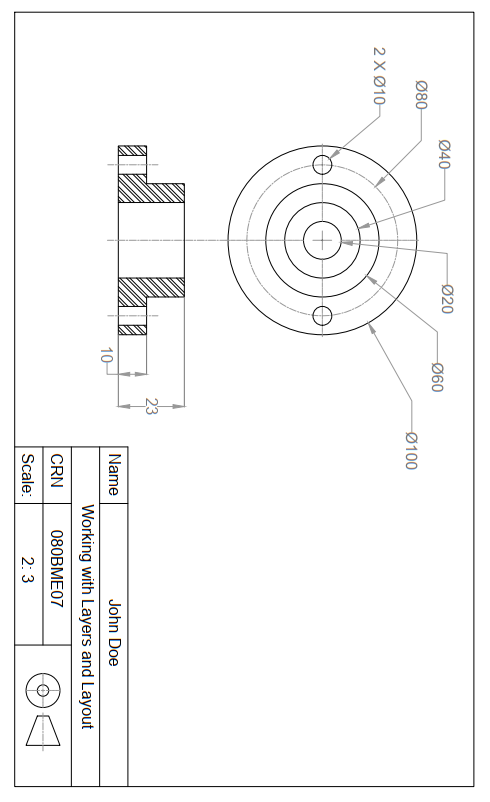
\includegraphics[scale = 0.8]{gfx/l5t1.PNG}
\end{center}
\subsection{Plot a layout in similar fashion to task 5.1 for task 4.3. The dimensions for the  title block is provided below.}
\begin{center}
	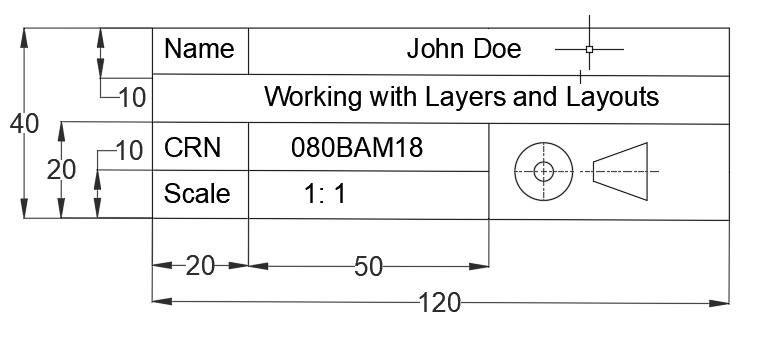
\includegraphics[scale = 0.7]{gfx/l5t2.PNG}
\end{center}
%lab 6
\section{Lab 6: 3D Modelling I: Modelling with primitive entities}
\foreach \n in {1,...,3}{
	\subsection{Model the solid object given in the figure below.}
	\begin{center}
		\includegraphics[width = 12cm, height = 12cm]{gfx/l6t\n.PNG}
	\end{center}
}
%lab 7
\section{Lab 7: 3D Modelling II: Modelling with custom sketch regions}
\foreach \n in {1,...,4}{
	\subsection{Model the solid object given in the figure below.}
	\begin{center}
		\includegraphics[width = 12cm, height = 12cm]{gfx/l7t\n.PNG}
	\end{center}
}
\end{document}